% Paquets généraux
\documentclass[a4paper,12pt,titlepage]{article}
\usepackage[T1]{fontenc}
\usepackage[utf8]{inputenc}
\usepackage[french]{babel}
\usepackage[gen]{eurosym}
%\usepackage[dvips]{graphicx}
\usepackage{fancyhdr}
\usepackage{pdfpages} 
\usepackage{multido}
\usepackage{hyperref}
%\usepackage{textcomp}
%\usepackage{aeguill}
\usepackage{schemabloc}
\usepackage[bitstream-charter]{mathdesign}
\usepackage{minted}

\newcommand{\id}{71}
\newcommand{\nom}{Théorie des mécanismes}
\newcommand{\sequence}{04}
\newcommand{\nomsequence}{Liaisons entre les solides}
\newcommand{\num}{02}
\newcommand{\type}{KH}
\newcommand{\descrip}{Liaisons équivalentes, hyperstatisme, liaisons en série et en parallèle, théorie des graphes}
\newcommand{\competences}{B2-12: Proposer une modélisation des liaisons avec leurs caractéristiques géométriques. \\ &  B2-13: Proposer un modèle cinématique paramétré à partir d'un système réel, d'une maquette numérique ou d'u \\ &  B2-17: Simplifier un modèle de mécanisme. \\ &  B2-18: Modifier un modèle pour le rendre isostatique. \\ &  C1-04: Proposer une démarche permettant d'obtenir une loi entrée-sortie géométrique.  \\ &  C2-05: Caractériser le mouvement d'un repère par rapport à un autre repère. \\ &  C2-06: Déterminer les relations entre les grandeurs géométriques ou cinématiques. }
\newcommand{\nbcomp}{7}
\newcommand{\systemes}{}
\newcommand{\systemesnum}{}
\newcommand{\systemessansaccent}{}
\newcommand{\ilot}{2}
\newcommand{\ilotstr}{02}
\newcommand{\dossierilot}{\detokenize{Ilot_02 }}


\newcommand{\auteurun}{Renaud Costadoat}
\newcommand{\auteurdeux}{Françoise Puig}
\newcommand{\institute}{Lycée Dorian}


\usepackage{color}
\usepackage{xcolor}
\usepackage{colortbl}
\usepackage{helvet}
\usepackage[frenchmath]{newtxsf} % for sans serif symbols
\renewcommand{\familydefault}{\sfdefault}
%\usepackage{amsfonts}
%\usepackage{amsmath}
%\usepackage{lmodern}
\usepackage{mathastext}
%\usepackage{xspace}
\usepackage{varioref}
\usepackage{tabularx}
%\usepackage{floatflt}
\usepackage{graphics}
\usepackage{wrapfig}
\usepackage{textcomp}
\usepackage{tikz}
\usepackage{wrapfig}
\usepackage{gensymb}
\usepackage[european]{circuitikz}
\usetikzlibrary{babel}
\usepackage{ifthen}
\usepackage{cancel}
\usepackage{etoolbox}
\usepackage{multirow}
%\usepackage{boxedminipage}
\definecolor{gris25}{gray}{0.75}
\definecolor{bleu}{RGB}{18,33,98}
\definecolor{bleuf}{RGB}{42,94,171}
\definecolor{bleuc}{RGB}{231,239,247}
\definecolor{rougef}{RGB}{185,18,27}
\definecolor{rougec}{RGB}{255,188,204}%255,230,231
\definecolor{vertf}{RGB}{103,126,82}
\definecolor{vertc}{RGB}{220,255,191}
\definecolor{forestgreen}{rgb}{0.13,0.54,0.13}
\definecolor{blcr}{rgb}{0.59,0.69,0.84}
\definecolor{blfr}{rgb}{0.32,0.51,0.75}
\definecolor{orfr}{rgb}{0.90,0.42,0.15}
\definecolor{orcr}{rgb}{0.90,0.65,0.50}
\definecolor{orangef}{rgb}{0.659,0.269,0.072}
\definecolor{orange}{rgb}{0.58,0.35,0.063}
\definecolor{orangec}{rgb}{0.43,0.32,0.25}
\definecolor{rcorrect}{rgb}{0.6,0,0}
\definecolor{sequence}{rgb}{0.75,0.75,0.75}
\definecolor{competences}{rgb}{0.61,0.73,0.35}
\definecolor{grisf}{HTML}{222222}
\definecolor{grisc}{HTML}{636363}
\definecolor{normal}{HTML}{4087c4}
\definecolor{info}{HTML}{5bc0de}
\definecolor{success}{RGB}{92,184,92}
\definecolor{warning}{RGB}{240,173,78}
\definecolor{danger}{RGB}{217,83,79}
\hypersetup{                    % parametrage des hyperliens
    colorlinks=true,                % colorise les liens
    breaklinks=true,                % permet les retours à la ligne pour les liens trop longs
    urlcolor= blfr,                 % couleur des hyperliens
    linkcolor= orange,                % couleur des liens internes aux documents (index, figures, tableaux, equations,...)
    citecolor= forestgreen                % couleur des liens vers les references bibliographiques
    }

% Mise en page
\pagestyle{fancy}

\setlength{\hoffset}{-18pt}

\setlength{\oddsidemargin}{0pt} 	% Marge gauche sur pages impaires
\setlength{\evensidemargin}{0pt} 	% Marge gauche sur pages paires
\setlength{\marginparwidth}{00pt} 	% Largeur de note dans la marge
\setlength{\headwidth}{481pt} 	 	% Largeur de la zone de tête (17cm)
\setlength{\textwidth}{481pt} 	 	% Largeur de la zone de texte (17cm)
\setlength{\voffset}{-18pt} 		% Bon pour DOS
\setlength{\marginparsep}{7pt}	 	% Séparation de la marge
\setlength{\topmargin}{-30pt} 		% Pas de marge en haut
\setlength{\headheight}{35pt} 		% Haut de page
\setlength{\headsep}{20pt} 		% Entre le haut de page et le texte
\setlength{\footskip}{30pt} 		% Bas de page + séparation
\setlength{\textheight}{700pt} 		% Hauteur de l'icone zone de texte (25cm)
\setlength\fboxrule{1 pt}
\renewcommand{\baselinestretch}{1}
\setcounter{tocdepth}{1}
\newcommand{\cadre}[2]
{\fbox{
  \begin{minipage}{#1\linewidth}
   \begin{center}
    #2\\
   \end{center}
  \end{minipage}
 }
}

\newcounter{num_quest} \setcounter{num_quest}{0}
\newcounter{num_rep} \setcounter{num_rep}{0}
\newcounter{num_cor} \setcounter{num_cor}{0}

\newcommand{\question}[1]{\refstepcounter{num_quest}\par
~\ \\ \parbox[t][][t]{0.15\linewidth}{\textbf{Question \arabic{num_quest}}}\parbox[t][][t]{0.93\linewidth}{#1}\par
}


\newcommand{\reponse}[1]
{\refstepcounter{num_rep}
\noindent
\rule{\linewidth}{.5pt}
\textbf{Question \arabic{num_rep}:}
\multido{\i=1+1}{#1}{~\ \\}
}

\newcommand{\cor}
{\refstepcounter{num_cor}
\noindent
\rule{\linewidth}{.5pt}
\textbf{Question \arabic{num_cor}:} \\
}

\newcommand{\titre}[1]
{\begin{center}
\cadre{0.8}{\huge #1} 
\end{center}
}


% En tête et pied de page
\fancypagestyle{normal}{%
  \fancyhf{}
\lhead{\nom}
\rhead{
\includegraphics[width=2cm]{../../img/logo}\hspace{2pt}}
\ifdef{\auteurdeux}{\lfoot{\auteurun,\auteurdeux}}{\lfoot{\auteurun}}
\cfoot{Page \thepage}}

\fancypagestyle{correction}{%
  \fancyhf{}
  \lhead{\colorbox{danger}{\begin{minipage}{0.65\paperwidth} \textcolor{white}{\textbf{Correction}} \end{minipage}} }
  \rhead{
\includegraphics[width=2cm]{../../img/logo}}
  \ifdef{\auteurdeux}{\lfoot{\auteurun,\auteurdeux}}{\lfoot{\auteurun}}
  \rfoot{\colorbox{danger}{\begin{minipage}{0.5\paperwidth} \begin{flushright}\textcolor{white}{\textbf{Correction}}\end{flushright} \end{minipage}} }}

\renewcommand{\footrulewidth}{0.4pt}

\usepackage{eso-pic}
\newcommand{\BackgroundPic}{%
\put(0,0){%
\parbox[b][\paperheight]{\paperwidth}{%
\vfill
\begin{center}
\hspace{0.5cm}\vspace{0.5cm}

\includegraphics[width=\paperwidth,height=\paperheight,%
keepaspectratio]{../../img/fond3}%
\end{center}
\vfill
}}}

\newcommand{\BackgroundPicdeux}{%
\put(25,-30){%
\parbox[b][\paperheight]{\paperwidth}{%
\vfill
\begin{center}

\includegraphics[width=\paperwidth,height=\paperheight,%
keepaspectratio]{../../img/fond4}%
\end{center}
\vfill
}}}

\begin{document}

\pagestyle{empty}

\vspace*{-3\baselineskip}

\AddToShipoutPicture*{\BackgroundPic}

\ifdef{\auteurdeux}{\begin{tabular}{>{\columncolor{gray!00}}m{.3\linewidth} m{.3\linewidth} >{\columncolor{gray!00}}m{.3\linewidth}}
Séquence : \sequence &  \multirow{3}{*}{\hspace{1cm}
\includegraphics[height=1.5cm]{../../img/logo}} &  \begin{flushright} \multirow{4}{*}{\hspace{1cm}\includegraphics[height=4cm]{img/qrcode}}\end{flushright}\\
Document : \type\num \\
 \institute \\
 \auteurun\\
 \auteurdeux
\end{tabular}}{\begin{tabular}{>{\columncolor{gray!00}}m{.3\linewidth} m{.3\linewidth} >{\columncolor{gray!00}}m{.3\linewidth}}
Séquence : \sequence &  \multirow{3}{*}{\hspace{1cm}
\includegraphics[height=1.5cm]{../../img/logo}} &  \begin{flushright} \multirow{4}{*}{\hspace{1cm}\includegraphics[height=4cm]{img/qrcode}}\end{flushright}\\
Document : \type\num \\
 \institute \\
 \auteurun
\end{tabular}}

\vspace{1cm}

\ifdef{\prive}{\begin{center}\colorbox{danger}{\Huge{Avec Correction}}\end{center}}{}

\begin{center}\huge{\nom}\end{center}

\vspace{2cm}

\ifdef{\imagedeux}{\begin{minipage}{0.49\linewidth}}{}
\begin{center}\includegraphics[height=5cm]{/home/renaud/Documents/Renaud/GitHub/django_education/systemes/\imageun}\end{center}
\ifdef{\imagedeux}{\end{minipage}\hfill
\begin{minipage}{0.49\linewidth}
\begin{center}\includegraphics[height=5cm]{/home/renaud/Documents/Renaud/GitHub/django_education/systemes/\imagedeux}\end{center}
\end{minipage}}{}

\vspace{5cm}


\begin{tabular}{p{.15\linewidth} >{\columncolor{white}}p{.8\linewidth}}
    \rowcolor{gray!20}
    Référence & S\sequence\ - \type\num \\
    Compétences & \competences \\
 	\rowcolor{gray!20}
    Description & \descrip \\
    Système & \systemes
  \end{tabular}

\newpage

\AddToShipoutPicture{\BackgroundPicdeux}

\pagestyle{normal}

\section{Etude d'un essai de traction}

\subsection{Essai continu}

\begin{figure}[!h]
 \begin{minipage}{0.6\linewidth}
Un essai de traction est utilisé afin de caractériser le comportement d'un  matériau métallique. Dans cet exemple, on choisiera un acier dont la désignation est X2CrNiMo15-8-1.

Cet essai de traction est effectué sur une éprouvette cylindrique dont le diamètre initial est D0=10mm et la longueur initiale est L0=50mm.

Après la rupture de l'éprouvette, le diamètre de la section de rupture est Df=6,9mm.

La courbe de l'effort F en fonction de la déformation conventionnelle (exprimée en \%) est donnée ci-dessous.

\vspace{1cm}

\centering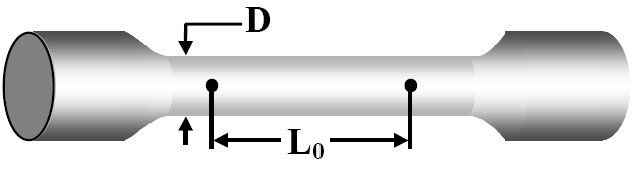
\includegraphics[width=0.9\linewidth]{img/eprouvette.png}
  \caption{Eprouvette de traction}
  \label{img:image1}
 \end{minipage}
\hfill
 \begin{minipage}{0.35\linewidth}
  \centering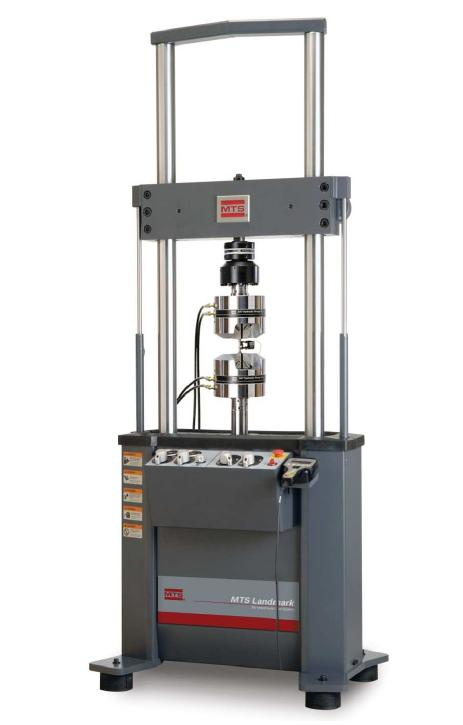
\includegraphics[width=\linewidth]{img/traction.jpg}
  \caption{Machine de traction}
  \label{img:image2}
 \end{minipage}
\end{figure}

\begin{figure}[!h]
  \centering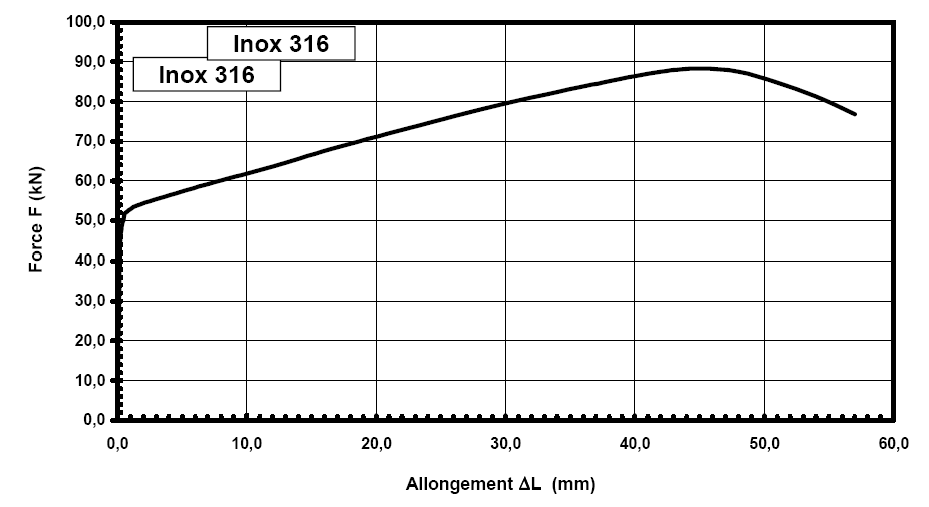
\includegraphics[width=\linewidth]{img/essai1.png}
  \caption{Courbe conventionnelle de l'essai de traction}
  \label{img:image3}
\end{figure}

 
 \begin{figure}[!h]
 \begin{minipage}{0.4\linewidth}
\paragraph{Question 1 :} Déterminez, à l'aide de la courbe conventionnelle de traction, les caractéristiques suivantes :
\begin{itemize}
 \item Limite conventionnelle d'élasticité à 0,2\% de déformation plastique $Rp_{0,2\%}$,
 \item Résistance maximale à la rupture par traction $Rm$,
 \item Allongement à rupture pour cent $A\%$.
\end{itemize}
 \end{minipage}
\hfill
 \begin{minipage}{0.59\linewidth}
  \centering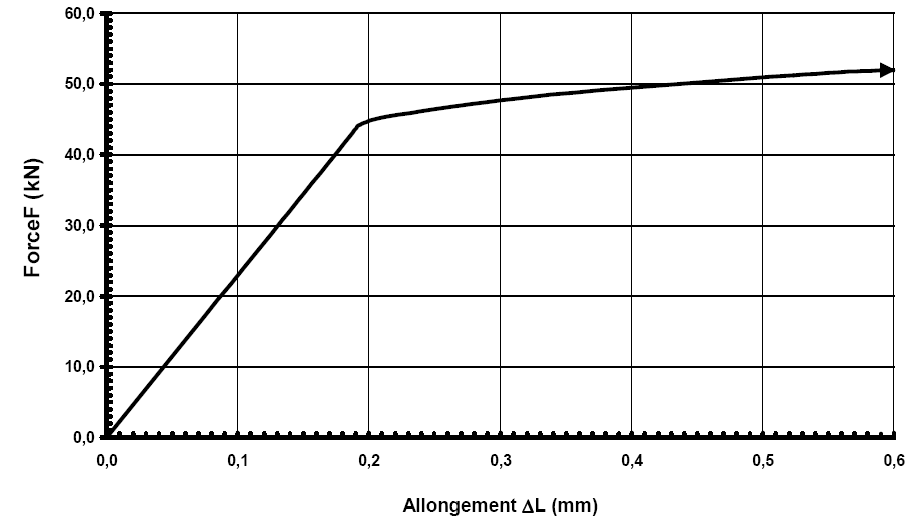
\includegraphics[width=0.8\linewidth]{img/essai2.png}
  \caption{Zoom sur l'origine de la courbe conventionnelle}
  \label{img:image4}
 \end{minipage}
\end{figure}

\paragraph{Question 2 :} D'après les données de départ, déterminez le coefficient de striction exprimé en pour cent $Z\%$.

\subsection{Evaluation de la fragilité}

Il existe deux façons de déterminer une évaluation de la fragilité d'un matériau:
\begin{itemize}
 \item par un essai de traction,
 \item par un essai de flexion-choc Charpy.
\end{itemize}

\paragraph{Question 3 :} A l'aide du résultat présenté sur la figure \ref{img:image3} donner une valeur permettant de caractériser la fragilité du matériau. Tracer sur la figure \ref{img:image3} en vert la courbe correspondant à un matériau moins fragile et en rouge celle d'un matériau plus fragile.

La suite va utiliser l'autre moyen d'évaluer la fragilité (ou son contraire: la résilience/tenacité) d'un matériau.

\section{Essai de résilience}

La résilience caractérise la capacité d'un matériau à absorber les chocs sans se rompre. Ce risque est amplifié aux basses températures. 

 \begin{figure}[!h]
 \begin{minipage}{0.45\linewidth}
Pour le test de résilience, la taille de l'éprouvette est normalisée (55x10x10 mm et entaille en U au milieu sur une hauteur de 5 mm).
 \end{minipage}
\hfill
 \begin{minipage}{0.45\linewidth}
  \centering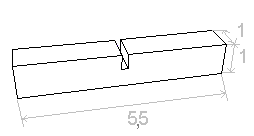
\includegraphics[width=0.7\linewidth]{img/eprouvette_U.png}
  \caption{Eprouvette pour un essai de résilience}
  \label{img:image5}
 \end{minipage}
\end{figure}

\paragraph{Question 1 :} Déterminer la section S de l'éprouvette au niveau de l'entaille.

 \begin{figure}[!h]
 \begin{minipage}{0.5\linewidth}
\centering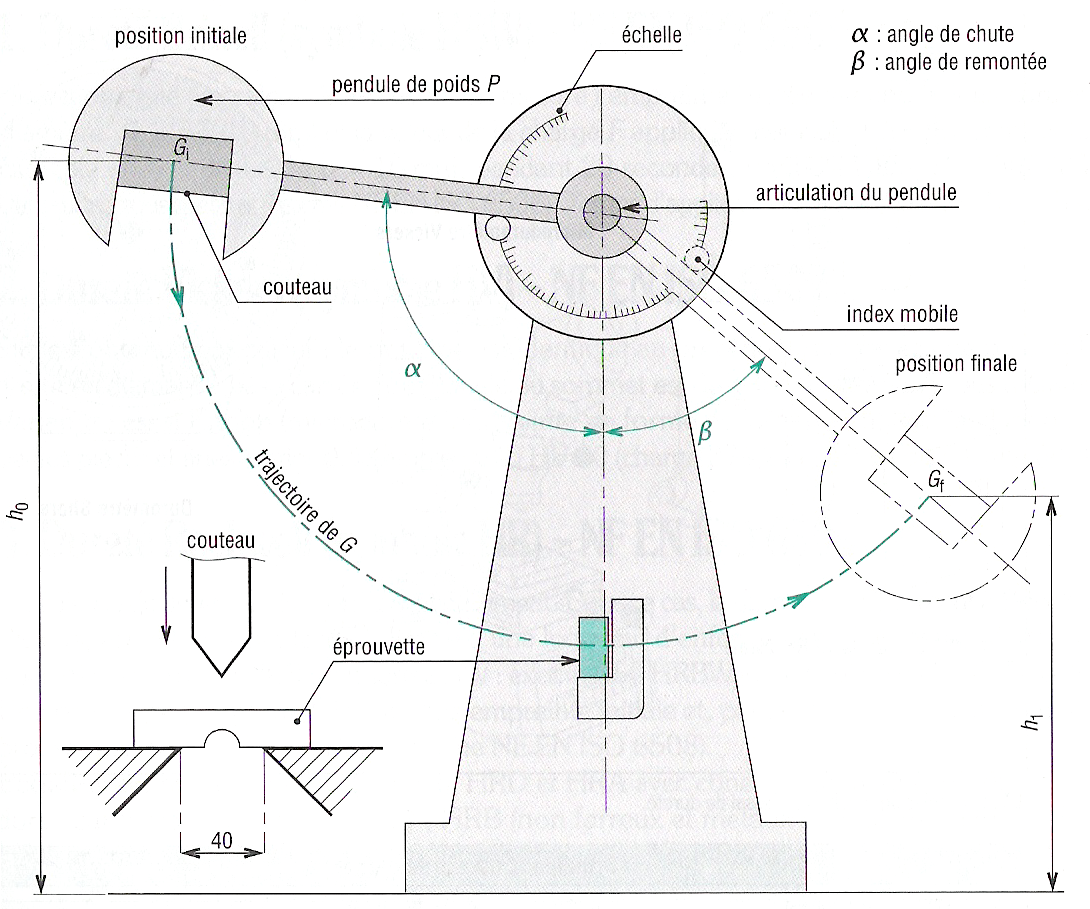
\includegraphics[width=0.7\linewidth]{img/mouton.png}
  \caption{\og Mouton de Charpy \fg}
  \label{img:image6}
 \end{minipage}
\hfill
 \begin{minipage}{0.49\linewidth}
Pour le test de résilience, la machine est appelée pendule \og Mouton de Charpy \fg.

La manipulation consiste à :
\begin{enumerate}
 \item relever le marteau (masse contenant le couteau) à une certaine hauteur,
 \item placer l'éprouvette au niveau le plus bas du passage du marteau,
 \item lâcher la masse.
\end{enumerate}
 \end{minipage}
\end{figure}

\newpage

Le couteau, dans sa course, vas percuter l'éprouvette et la casser, y perdant une partie de son énergie gagnée grâce à se mise en hauteur. L'énergie absorbée par l'éprouvette est égale à la perte d'énergie du marteau, donc à sa perte d'énergie potentielle.

 \begin{figure}[!h]
 \begin{minipage}{0.4\linewidth}
\begin{itemize}
 \item au départ : $W_0 = m.g.H_0$,
 \item après le test : $W_1 = m.g.H_1$,
\end{itemize}
 \end{minipage}
\hfill
 \begin{minipage}{0.59\linewidth}
\begin{itemize}
 \item $H_0 = 1 m$,
 \item $G = 9.81 m.s^{-2}$,
 \item $m = 5 kg$, il s'agit de la masse du marteau.
\end{itemize}
 \end{minipage}
\end{figure}

Alors, $\Delta W = m.g.(H_0 - H_1)$, ainsi une image de la fragilité peut être déterminée.

L'expérience va être réalisée sur deux éprouvettes réalisée dans le même matériau, mais dont l'un aura été écroui. L'écrouissage d'un métal est le durcissement d'un métal sous l'effet de sa déformation plastique (définitive).

\begin{itemize}
 \item Matériau non écroui : $H_1=0.18 m$,
 \item Matériau écroui : $H_1=0.75 m$.
\end{itemize}

\paragraph{Question 2 :} Déterminer l'image de la résilience $\Delta W/S$ en $daJ.cm^{-2}$ pour ces deux éprouvettes, où S est la section de l'éprouvette au niveau de l'entaille.

\section{Essai de fatigue}

Les caractéristiques mécaniques peuvent aussi concerner des chargements répétés afin de caractériser la fatigue d'un matériau.

\begin{figure}[!h]
\centering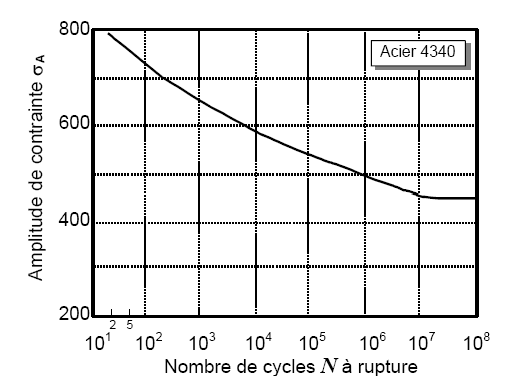
\includegraphics[width=0.6\linewidth]{img/essai3.png}
  \caption{Résultat d'un essai de fatigue sur cette éprouvette}
  \label{img:image7}
\end{figure}

\paragraph{Question 1 :} Déterminez le nombre de cycle (le nombre d'alternance) que peut subir la pièce, soumise à des efforts d'amplitude 500Mpa, avant sa rupture.

\paragraph{Question 2 :} Déterminez la limite d'endurance $\sigma_D$ de cet acier.

\begin{figure}[!h]
 \centering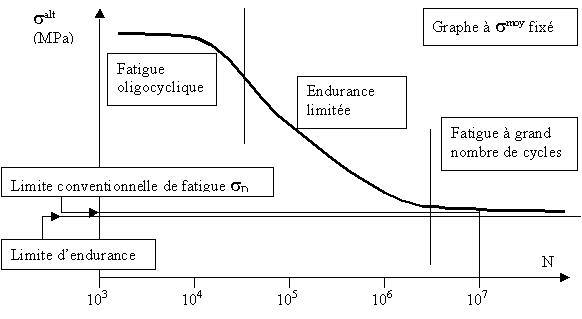
\includegraphics[width=0.8\linewidth]{img/essai4.png}
  \caption{Aide à la lecture d'un essai de fatigue}
  \label{img:image8}
\end{figure}

\ifdef{\public}{\end{document}}{}

\cleardoublepage

\pagestyle{correction}

\newpage


\paragraph{Question 1:}

$\epsilon=\frac{\Delta L}{L_0}=0,2\%=0,2.10^{-2}=\frac{\Delta L}{50}$, donc $\Delta L=50.0,2.10^{-2}=0,1mm$

$F_{p0,2\%}=46kN$, donc $R_{p0,2\%}=\frac{46000}{\pi.\frac{10^2}{4}}=\frac{460.4}{\pi}=585,7MPa$.

~\

$F_m=88kN$, donc $R_m=\frac{880.4}{\pi}=1,12GPa$

~\

$A\%=\frac{57}{50}=1,14$.

\paragraph{Question 2:}

$Z\%=\frac{S_0-S_u}{S_0}.100=\frac{d_0^2-d_f^2}{d_0^2}.100=52,39\%$

\paragraph{Question 3:}

$Z=0,52>0,1$, donc le matériau n'est pas fragile.

L'aire sous la courbe est environ: $a=\frac{70.10^3}{\pi.10^2}.\frac{60}{50}=267,4MPa$, c'est une image de la fragilité.

\begin{center}
 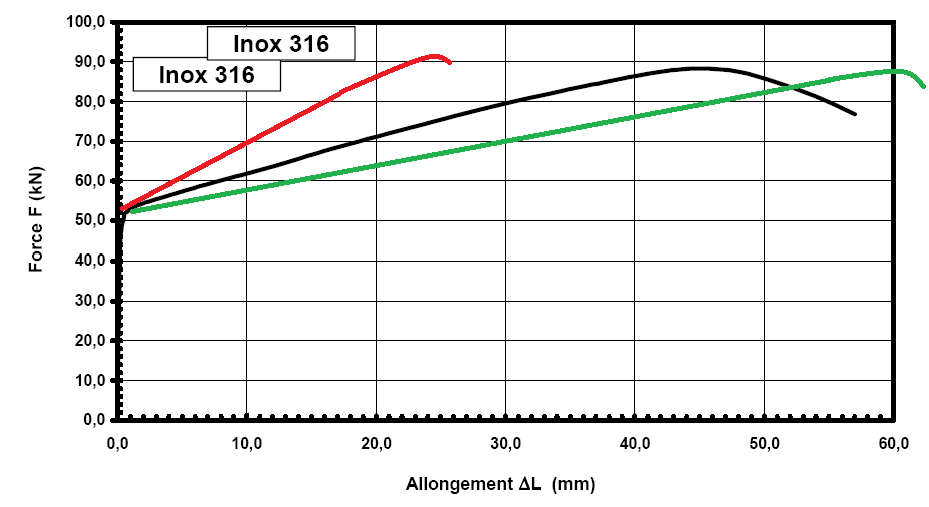
\includegraphics[width=0.8\linewidth]{img/essai1_cor}
\end{center}

\subsection{Essai de résilience}

\paragraph{Question 1:} $S=10.5=50mm^2$

\paragraph{Question 2:} ~\

\begin{itemize}
 \item Matériau non-écroui: $\frac{\Delta W}{S}=\frac{5.9,81.(1-0,18)}{0,5}=80,442=8,04daJ.cm^{-2}$,
 \item Matériau écroui: $\frac{\Delta W}{S}=\frac{5.9,81.(1-0,75)}{0,5}=24,525=2,45daJ.cm^{-2}$.
\end{itemize}

\subsection{Essai de fatigue}

\paragraph{Question 1:} A $500Mpa$, il y a rupture au bout de $10^6$ cycles.

\paragraph{Question 2:} $\sigma_D=450MPa$.

\end{document}
